% results_visualization.tex
\subsection{Visualization}

Beyond the \texttt{sfa\_corplot()} similarity heatmaps
(Figure~\ref{fig:corplot}, left and right panels) and the
\texttt{plot()} scree and loading plots (Figures~\ref{fig:scree}
and~\ref{fig:loadings}), \texttt{sfa\_itemplot()} maps items into two
dimensions by t-SNE \citep{vandermaaten-hinton-2008}, UMAP, PCA, or
classical MDS:

{\scriptsize
\begin{verbatim}
> for (m in c("tsne", "umap", "pca", "mds")) {
+   sfa_itemplot(fit, method = m, seed = 42, legend = (m == "tsne"))
+ }
\end{verbatim}
}

In all four projections (Figure~\ref{fig:itemmap}), Neuroticism,
Conscientiousness, and Openness items form compact, separated
neighborhoods, whereas Extraversion and Agreeableness items interleave in
a shared sociability region---a geometric preview of the factor
solution's MR2/MR5 blending and the congruence results that follow.

\begin{figure}[H]
\centering
\captionsetup{justification=raggedright,singlelinecheck=false}
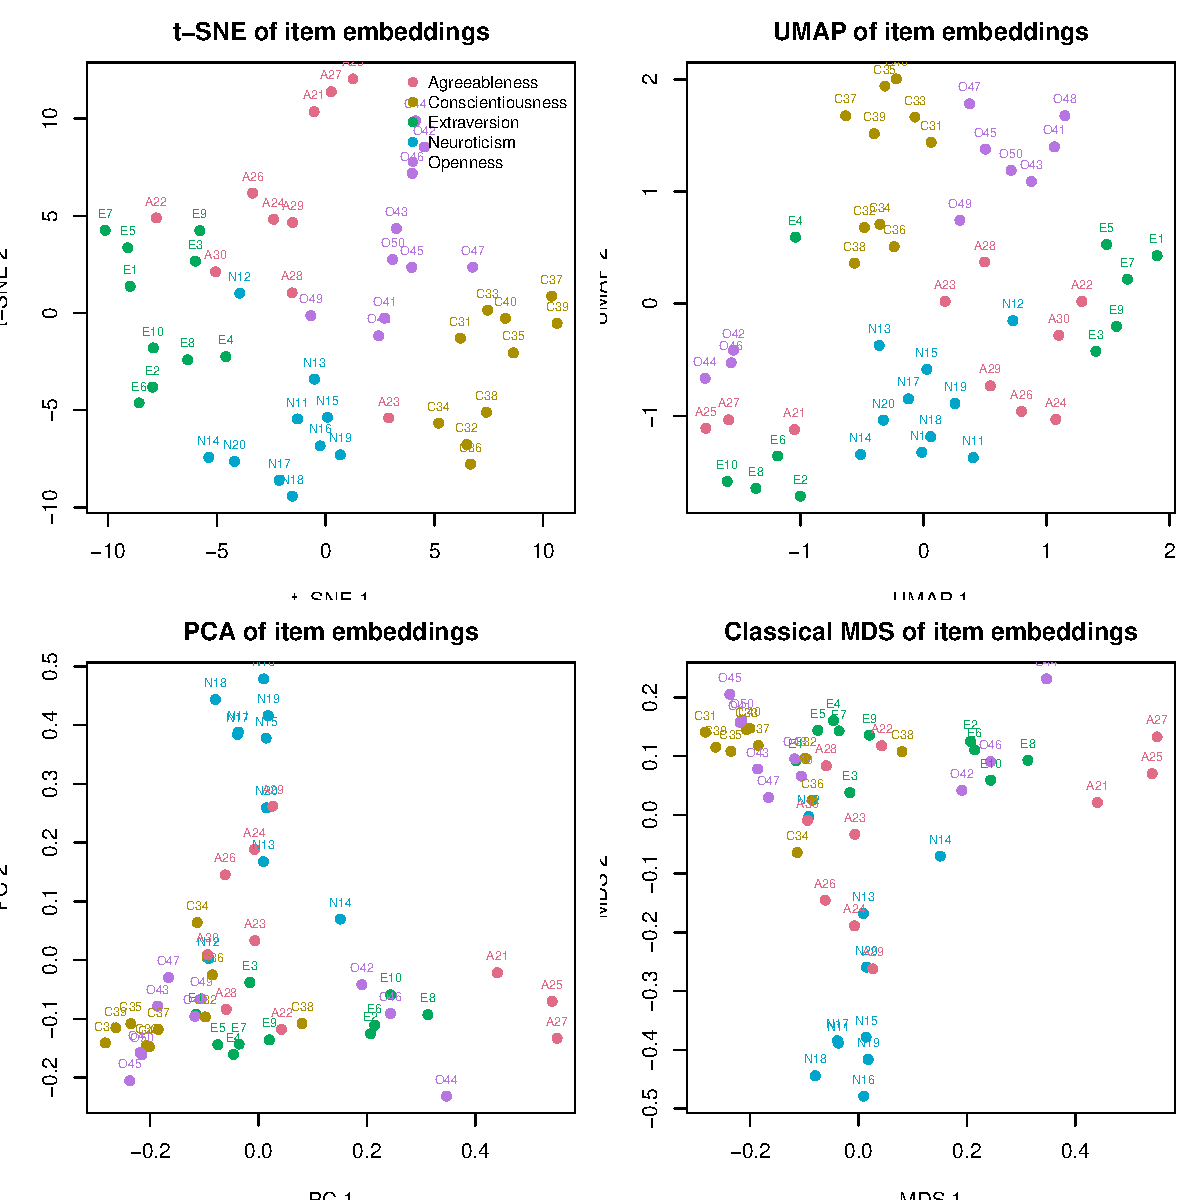
\includegraphics[width=0.8\textwidth]{figures/itemmap.pdf}
\caption{Two-dimensional item maps of the 50 item embeddings produced by
\texttt{sfa\_itemplot()}: t-SNE (top left), UMAP (top right), PCA (bottom
left), and classical MDS (bottom right), with items colored by theoretical
domain. Neuroticism, Conscientiousness, and Openness items cluster tightly
in all four projections; Extraversion and Agreeableness items interleave.}
\label{fig:itemmap}
\end{figure}
